\documentclass[10pt]{article}
\author{Tom Lemberg and Will Sun}
\title{CrowdTruth: Crowdsourcing Political Fact-Checking}
\date{October 11, 2012}

\usepackage{graphicx}
\usepackage[margin=1in]{geometry}                
\geometry{letterpaper}                  
\usepackage{graphicx}
\usepackage{amsmath, amssymb, amsthm}
\usepackage{hyperref}

\begin{document}
\maketitle

\section{Introduction}

\noindent
With the general elections less than a month away and candidate debates taking place nearly every week, we decided it would be interesting to try to apply crowdsourcing principles to political fact-checking. Currently websites like \url{http://www.factcheck.org} and \url{http://www.politifact.com} analyze political statements and determine how truthful they are through the use of expert investigation. These experts are paid at a high rate and are devoted to producing quality results. Using TurKit and workers on Amazon Mechanical Turk, we developed CrowdTruth, an application that strives to synthesize crowdsourced analysis to provide meaningful annotations of text.

\section{Design}
\noindent
CrowdTruth employs a variant of the standard ``Find-Fix-Verify'' model introduced by Bernstein \emph{et al.} (2010). We begin by identifying factual claims made in the text, verify these identifications, request sources to either prove or disprove a claim, and then vote on these sources. Here ``Fix'' essentially requires source identification. A diagram of our workflow is below: \\

\begin{center}
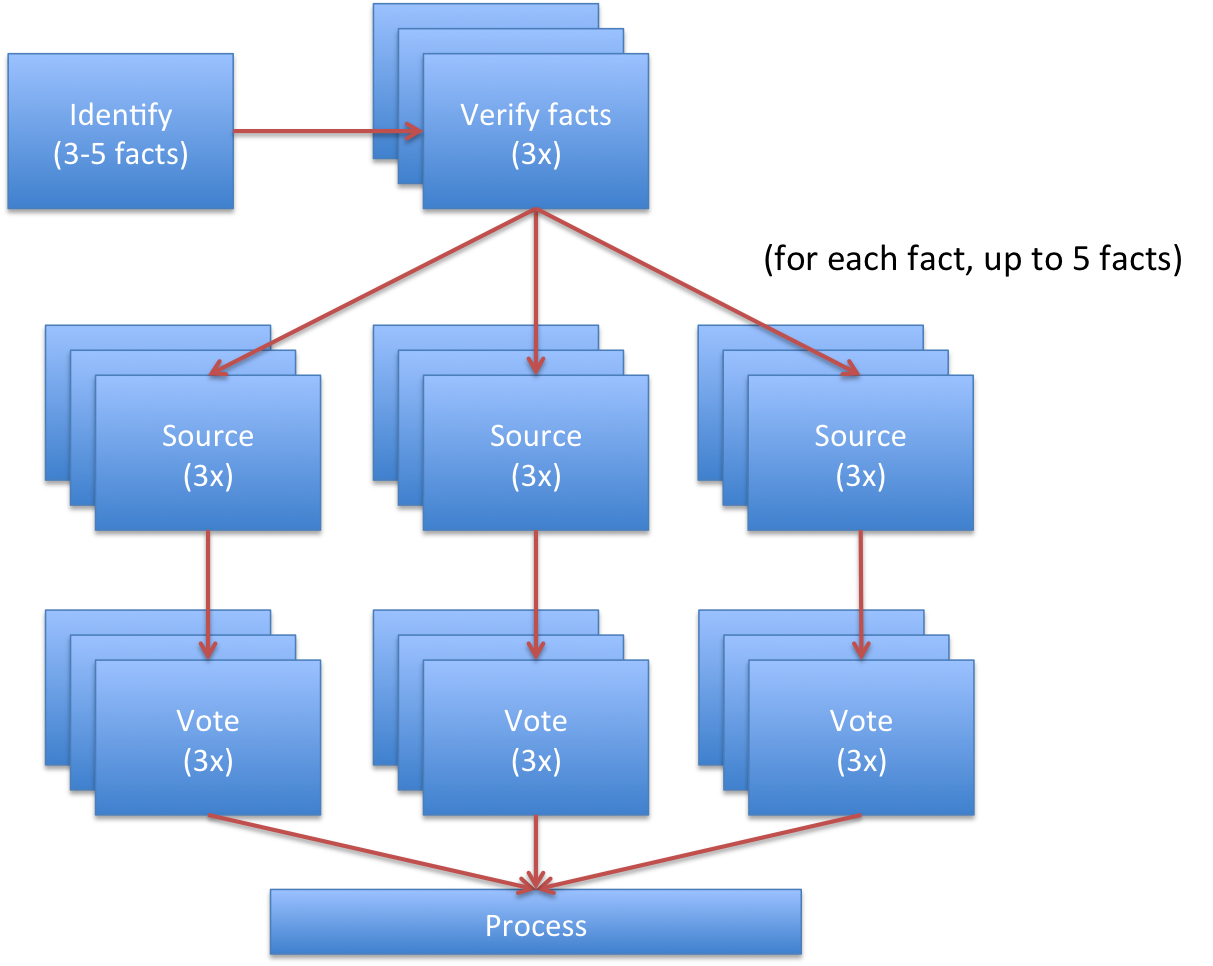
\includegraphics[width=4in]{flow.png}
\end{center}

\noindent
At the identify step, a user is directed to copy and paste 3-5 claims into the response boxes. The following verification step presents this set of claims to several users, asking them to identify whether each fact is an objective claim and a complete thought. This allows us to filter out text input that is not suited for our analysis. We then ask for 3 sources to prove or disprove each claim; each source requires a link, a description or excerpt, and a label whether it proves or disproves the fact. Finally, our voting step presents to several users a claim, a set of sources, and the request to (1) rate each source's validity on a scale of 1-10, (2) note whether the source is a duplicate, and (3) rate the overall fact's ``truth value'' on a scale of 1-10. Our code can be found at our Github repository (\url{http://github.com/wsun/crowdtruth}) and our sample visualization at \url{http://tjcs279.0fees.net/project2/doc.php#}.

\section{Results and Discussion}
\noindent
So far, we have run our entire flow on one excerpt from the recent presidential debate between Romney and Barack Obama (a second was in progress at the time of writing). We initially set our HIT rewards at \$.04, \$.02, \$.25, \$.10 for identify, verify, source, and vote respectively, but after hours of no work completed, we decided to increase our rewards significantly. Overall, the quality of results are promising, and with minor adjustments in our workflow, we are confident that this application can produce useful information. Below are two screenshots from the Romney excerpt analyzed: \\

\begin{center}
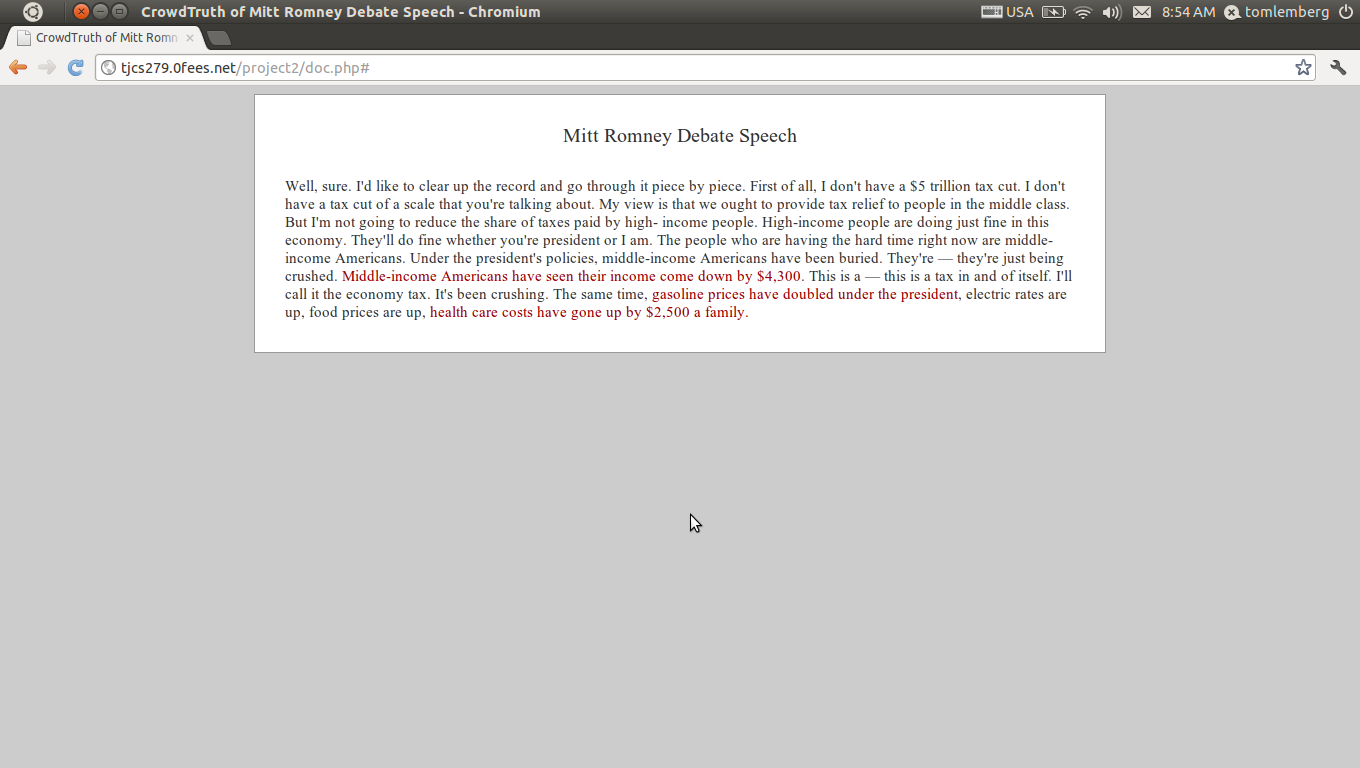
\includegraphics[width=6.5in]{ui1.png}
\end{center}

\begin{center}
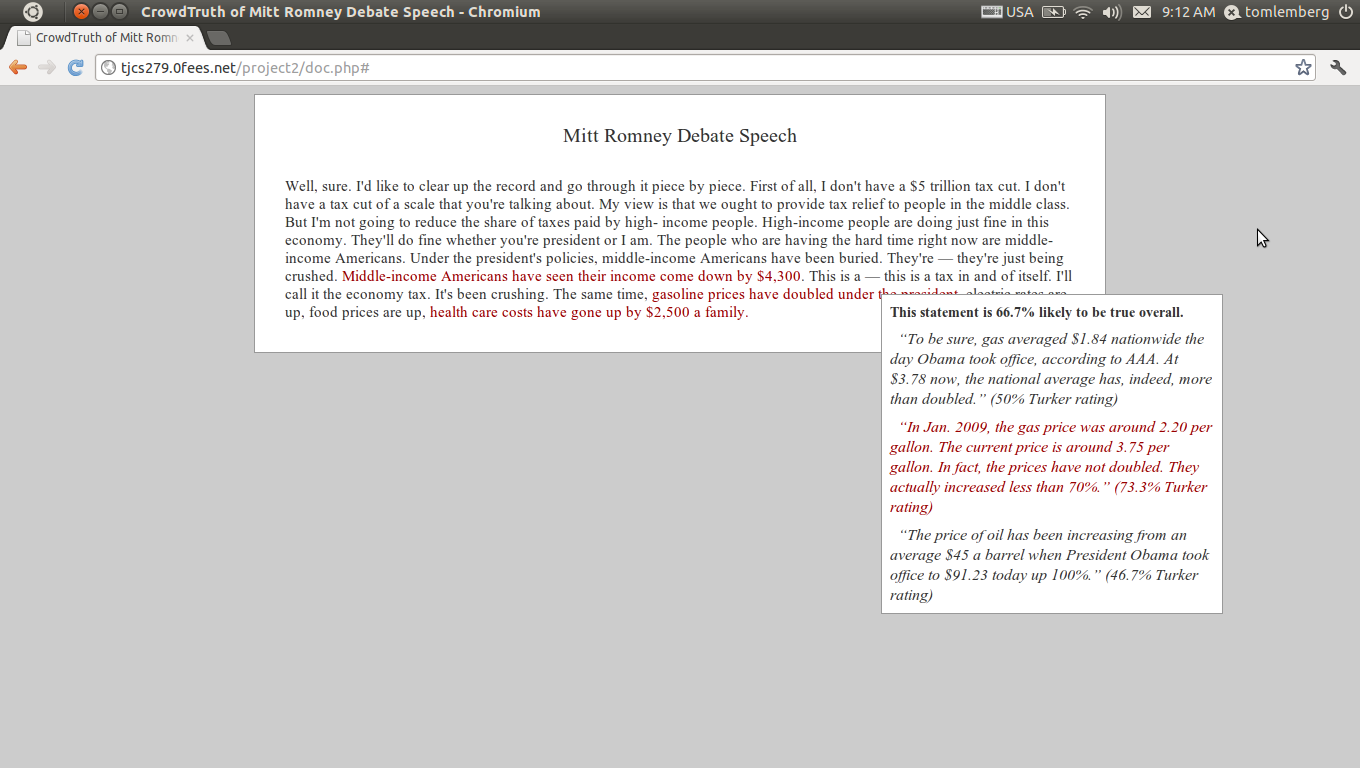
\includegraphics[width=6.5in]{ui2.png}
\end{center}

\noindent
Our three primary considerations for our application's output are \emph{accuracy}, \emph{speed}, and \emph{cost}. Though we likely would not be able to match professional fact-checkers in their accuracy and citations, we need our workers to produce results that aren't completely off. This we hope to ensure by building in verification steps. Speed and cost are areas in which our application can potentially beat a professional fact-checking unit: by crowdsourcing our tasks, we can parallelize \emph{and} save money by using non-experts. \\

\noindent
To maximize accuracy, we presented clear instructions for each task, including example facts or sources to guide users. We decided to omit the author of the excerpt in the identification stage, so as to minimize potential biases (though of course, depending on the passage, the author could be implicitly deterined), and also requested that users identify ``potentially incorrect factual claims''. We initially tested with ``factual claims,'' but decided that instructing users to find ``incorrect'' ones would not only better inform the user of the purpose of their work but also help bias our claims toward those that might be incorrect (which is preferable for our general purposes).Our verification steps are also critical toward maximizing accuracy; based on our verify results, we modify our result set accordingly. With 3 voters verifying a set of 3-5 facts from a passage, we throw out any fact that was identified by \emph{all} voters as not appropriate. Additionally, with 3 voters verifying a set of 3 sources, we throw out any source that has an average source quality rating of 1.25 and any source that has been marked by each voter as a duplicate; these thresholds can be modified to increase the quality of results, trading off with quantity. Though our current implementation uses 3 voters to verify a set of facts and 3 voters to verify a set of sources, we could increase this number at the expense of cost and speed. Finally, our implementation does not impose any qualification requirements whatsoever; having veteran Turkers from the United States alone would help.\\

\noindent
Optimizing for speed necessarily requires an effective parallel implementation of the work. We chose TurKit primarily because of its simple GUI and its crash-and-rerun debugging model. Moreover, TurKit seemed to support both iterative and parallel task completion. Unfortunately, the creator of TurKit removed the key \verb!fork()! command, which would allow multiple HITs to proceed in parallel. This meant that we were unable to parallelize our work, eliminating much of our application's advantage in speed. \\

\noindent
With respect to cost, from a time-based derivation of HIT rewards, we estimated it would take a few dollars to fact-check a short passage (1-2 paragraphs). However, due to time limitations and the above difficulties with parallelizing work, we were forced to significantly increase our rewards to compel work, ultimately costing nearly \$15 for a single passage. Even if our initial HIT reward level was used, spending a few dollars for a few paragraphs would not save much money compared to paying an expert for higher-quality results. \\

\noindent
Future work on this project could include improvements to our visualization to more effectively display our two 1-10 ratings (source validity and fact truth). Moreover, our current implementation is clumsy in the way it asks users to identify duplicate sources; we can automate this by actually examining each link. Ultimately, we would like to make this application available to users, so we would need to develop a web interface that allows people to upload documents and leverage their MTurk accounts to have work completed. \\

\noindent
Though the speed and cost are not significantly less than what an expert fact-checker would require, and the quality is not as high as an expert's analysis, CrowdTruth provides the additional benefit of sampling both a population opinion and the collective opinion of secondary sources. This also points to one of our limitations: CrowdTruth will never be able to use primary sources. Unlike Soylent, which took advantage of simple tasks, even our comparmentalized tasks imposed a high cognitive load on users - asking them to examine primary sources would be even harder. Overall, CrowdTruth offers an automated alternative to fact-checking.

\end{document}